\documentclass{article}

\usepackage[a4paper,left=18mm,right=18mm,top=20mm,bottom=18mm]{geometry}
\usepackage[italian]{babel}

\usepackage{titling}
\usepackage{graphicx}
\usepackage{subcaption}
\usepackage{float}
\usepackage{hyperref}


\title{Documentation for Software engineering project}
\author{Nicolas Anselmi, David Guzman Piedrahita and Marco Vinciguerra}

\begin{document}
\maketitle
\section{Project Plan}
\subsection{Introduction}
Il progetto prevede lo sviluppo di una mobile app per gestire la prenotazione di 
un negozio di parruccheria. C'è la possibilità di avere due tipi di utente (anche in entrambe le mdoalità):
un cliente e un padrone di negozio. La novità di questo progetto consiste nel fatto che è un tipo di sistema P2P in cui un utente può essere contemporaneamente cliente
e (se vuole) gestore. Questo modello di business è fatto anche da Uber in cui un autista può essere sia cliente che autista.
\\Il target della clientela è market driven in quanto il core business dell'azienda si basa su percentuali delle transazioni.
Il cliente ha la possibilità di prenotare diversi 
tipi di acconciatura direttamente senza interfacciarsi /chiamare direttamente il proprietario
del negozio ma tramite l'applicazione.Ogni tipologia di taglio selezionabile ha una durata e in base al tipo dei macchinari e delle risorse che devono essere utilizzate 
e può consentire un orario customizzabile di prenotazione 
da parte del cliente. 
\\I membri del team sono: Nicolas Anselmi, David Guzman Piedrahita e Marco Vinciguerra.

\subsection{Process model}
Il life cycle del progetto è agile, in particolare la tecnica utilizzata è SCRUM con
sprint di 5 giorni in quanto il tempo necessario per lo sviluppo è breve. Inoltre viene utilizzato un triage per
gestire i compiti (MoSCoW).
\\Inoltre viene applicato un modello di prototipazione incrementale in cui ad ogni git viene aggiunto una funzionalità al sito e deve essere sempre disponibile
su Github una versione funzionante del progetto.
\\Per accelerare il processo di apprendimento viene applicato anche il processo di pair programming, 
pratica molto utilizzata nei metodi AGILE.
\\Per quanto riguarda i requirements si utilizza il Kano Model.
Il periodo di sviluppo parte poco prima di Natale. Ogni giorno verso le 9 30 del mattino 
c'è un daily scrum tenuto dallo scrum master in cui si discutono le problematiche riscontrate durante 
il giorno precedente e le possibili soluzioni a queste.

\subsection{Organization of the project}
Il progetto, dovuto alla sua natura, deve intefacciarsi sia con utenti  che usufruiscono del servizio di prenotazione, sia da utenti che mettono a disposizioni i loro servizi commerciali.
Il team di sviluppo è composto dai succitati integranti. Per portare a termine l'applicazione, ci sono dei knowledge-gap che dovranno essere colmati tramite la lettura di documentazione e
l'uso di risorse online: particolarmente nel caso del framework Flutter per il frontend development.

\subsection{Standards, guidelines, procedures}
I principali linguaggi di programmazione del progetto saranno: python e dart, quest'ultimo
viene esteso tramite flutter.
Si usa i coding standards di flutter.
\\Per gestire l'assegnazione e il corretto sviluppo si usa un template di Notion per gestire i compiti.
\\Gli IDE che vengono utilizzati sono: VSC e terminale con VIM.

\subsection{Management activities}
Ogni settimana viene fatto un report sui progressi in corso fatti dal team di sviluppo per avere un'idea sull'avanzamento del progetto.
\\Le modifiche critiche del progetto devono essere accettate dal padrone della cartella (Marco Vinciguerra), le altre possono essere fatte 
liberamente.
\\Questi report, insieme alle decisioni definite negli scrum meeting, rappresentano la principale strategia per valutare velocemente lo status del progetto, e, 
di conseguenza, sono utili a fare course-correction.
\\Difatti, è proprio in questo modo che è previsto bilanciare l’equilibrio tra requirements e l’impegno necessario per soddisfarli.  
\subsection{Risks}
Il rischio principale è di non consegnare in tempo il progetto o di non consegnare un progetto perfettamente funzionante.
\subsection{Staffing}
I membri del team sono: Nicolas Anselmi, David Guzman Piedrahita e Marco.
\\Per provare a vedere come funziona il mestiere il ruolo dello SCRUM master cambia a rotazione e si parte dalla settimana 
che inizia col 13 dicembre. Il primo SCRUM master sarà David, la settimana dopo Nicolas e quella dopo Marco Vinciguerra e così via...
\\Sono 3 studenti di ingegneria del terzo anno.

\subsection{Methods and techiniques}
Per gestire gli sprint è stato utilizzato un template di Notion in quanto ha la possibilità di schedulare i task in base alla scadenza e in base ad un ordine gerarchico.
\\Per gestire la fase di testing si usa il tool better flutter tests che fa lui il testing sul framework Flutter. Il test viene scritto automaticamente dal tool e quindi 
non si applica fin da principio.
\\Per quanto riguarda la specifica dei requisiti si utilizza lo standard IEEE 830.
\\Il design pattern utilizzato è il delegation pattern.
\\Si utilizza Flutlab.io per convertire il modello fatto con Figma in codice sorgente Flutter, questa è una strategia model driven.
\\Si prevede l'uso di una strategia COTS per la scelta di diversi moduli o, più precisamente, widget di Flutter, che consentono di implementare velocemente
elementi UI classici, senza scrivergli da zero.
\\Per quanto riguarda i test di Dart si utilizza Dart unit testing e si utilizza il TDD e per garantire la continuos integration si usa Travis CI che partirà ad ogni 
Git e ogni 24 ore.
\\Per i database non si fa nessun tipo di testing e si utilizza Firebase  per creare e gestire il database delle prenotazioni.
\\La gestione delle modifiche viene svolta tenendo in conto le considerazione del punto 5 e, soprattutto, il punto 13.
\subsection{Quality assurance}
Per garantire la qualità del prodotto viene utilizzato lo standard ISO 9001.

\subsection{Work packages}
Alcuni dei sottoprogetti (work package) che sono stati definiti a priori.
\\ In viste della natura agile del progetto, questi work-package saranno estesi e modificati o evoluti nelle diverse iterazioni del life-cycle:
\begin{itemize}
    \item Fase di design di schemi UML
    \item Imparare ad utilizzare Flutter e dart
    \item Implementare l'applicazione con un'interfaccia grafica (front-end)
    \item Implementare la domain logic (back-end)
    \item Uso di un database
    \item Fare il testing sul prodotto
    \item Fare testing usando l'applicazioni in telefoni reali (non simulator)
\end{itemize}

\subsection{Resources}
Gli obiettivi di prototipazione proposti dal progetto in questione richiedono solo l'uso di computer adatti alla programmazione nei suddetti linguaggi e framework.
Dopo diverse iterazioni di prototipazione è prevista la possibilità di usare dei cloud-server che ricevano e gestiscano le richieste degli utenti tramite i loro client/app. 

\subsection{Budget and schedule}
Il tempo preventivato per il progetto è di circa 55 ore a testa, quindi in totale saranno richieste 150 ore.
\\In particolare si prevede che saranno richieste 30 ore per fare la documentazione, 10 ore per imparare Flutter e dart, 10 ore per implementarla
e le restanti ore i database e il testing.
\subsection{Changes}
Col tempo potrebbero cambiare le richieste da parte del cliente durante la fase di validazione di ogni processo.
\\Al supporto delle attività di change management vengono utilizzati i due tool usati anche per altri aspetti del progetto, ovvero: 
\\Github, che in questo caso funge da piattaforma per accettare o rifiutare le modifiche version-oriented e per consentire di usare il forked develpment; 
\\e Notion che, non essendo un tool specifico per lo sviluppo, serve invece a gestire l’organizzazione delle tempistiche e dei sotto-progetti a un livello di astrazione più alto.
\\I contenuti di questi tool, e i diversi report dei punti precedenti, servono come guida per la compilazione di un eventuale configuration management plan che conterrà una management section e activities. I documenti generati come risultato del punto 5 sono particolarmente utili per la management section.

\subsection{Delivery}
Il project plan verrà consegnato entro il 27 dicembre 2021
\\La consegna verrà fatta 5 giorni prima dell'esame orale di gennaio.
\subsection{People Management and Team Organization}
\subsection{Softare Quality}
\subsubsection{CMM}
Per quanto riguarda il CMM (Capaibility Maturity Model) esistono 5 livelli di maturità del software, essi sono:
\begin{itemize}
    \item Initial 
    \item Managed
    \item Defined
    \item Measurable
    \item Optimization
\end{itemize}
In questo progetto si punta ad utilizzare il terzo livello 3 (Defined) in cui ogni attività viene documentata
e standardadizzata per l'intera organizzazione del processo per il design, development e testing.

\subsubsection{ISO 9216}
Per quanto riguarda la product conformance si fa riferimento al seguente link: \url{https://www.geeksforgeeks.org/iso-iec-9126-in-software-engineering/}
\\Esso si basa sui 4 seguenti principi:
\begin{itemize}
    \item \textbf{Part 1: "Quality model"} 
    \item \textbf{Part 2: "External metrics"} 
    \item \textbf{Part 3: "Internal metrics"} 
    \item \textbf{Part 4: "Quality in use metrics"} 
\end{itemize}
Per chiarire meglio il concetto si fa riferimento al seguente grafico:
\\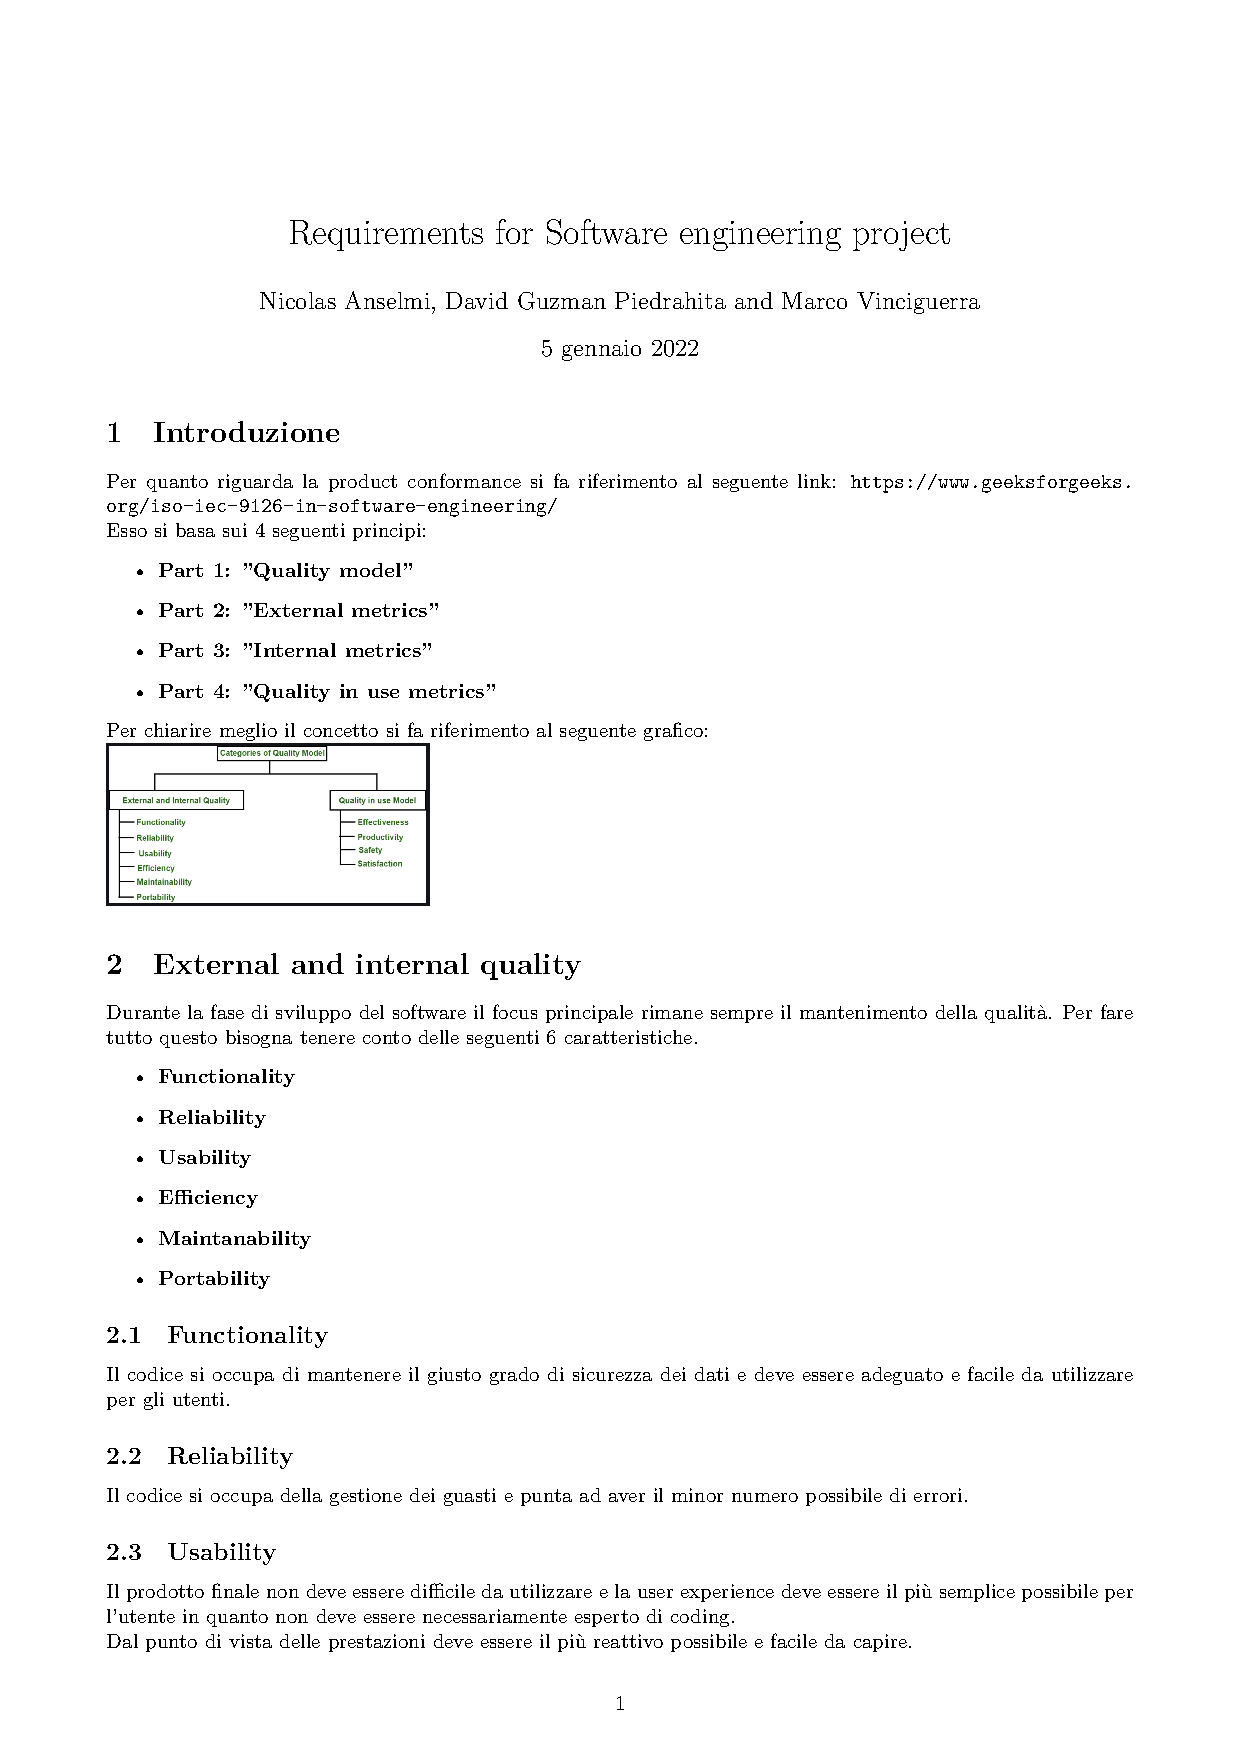
\includegraphics[scale = 0.25]{"Immagini/ISO9126.PNG"}
\section{External and internal quality}
Durante la fase di sviluppo del software il focus principale rimane sempre il mantenimento della qualità.
Per fare tutto questo bisogna tenere conto delle seguenti 6 caratteristiche.
\begin{itemize}
    \item \textbf{Functionality} 
    \item \textbf{Reliability} 
    \item \textbf{Usability} 
    \item \textbf{Efficiency} 
    \item \textbf{Maintanability} 
    \item \textbf{Portability} 
\end{itemize}

\subsection{Functionality}
Il codice si occupa di mantenere il giusto grado di sicurezza dei dati e deve essere adeguato e facile
da utilizzare per gli utenti.

\subsection{Reliability}
Il codice si occupa della gestione dei guasti e punta ad aver il minor numero possibile di errori.

\subsection{Usability}
Il prodotto finale non deve essere difficile da utilizzare e la user experience deve essere il più
semplice possibile per l'utente in quanto non deve essere necessariamente esperto di coding.
\\Dal punto di vista delle prestazioni deve essere il più reattivo possibile e facile da capire.

\subsection{Efficiency}
Si vuole creare il programma più efficiente possibile che utilizzi il minimo delle risorse del dispositivo
da cui si utilizza l'applicazione.

\subsection{Maintanability}
Il codice deve essere scritto nel modo più conforme alle regole di standard di programmazione per favorire
la leggibilità e la successiva manutenzione.

\subsection{Portability}
Il programma deve funziona su più piattaforme possibilil.

\section{Quality in use Model}
Si basa sulle seguenti 4 caratteristiche che si vuole soddisfare:
\begin{itemize}
    \item Effectiveness
    \item Productivity
    \item Safety
    \item Satisfaction
\end{itemize}
\subsection{Requirement Engeneering-IEE830}
\subsection{Software Architecture}
\subsection{Software Design}
\subsection{Software Testing}
\subsubsection{IEEE928}
Questo tipo di documento si occupa di specificare e documentare come avviene la fase di testing
del progetto. Questo documento rappresenta anche il test plan. Siccome stiamo facendo un tipo di
sviluppo di software AGILE i test non vengono fatti alla fine ma vengono svolti in contemporanea allo
sviluppo delle classi.
\\Viene svolto un tipo di sviluppo di tipo TDD in cui si scrivono le classi dei test in 
contemporanea (se non prima) delle classi che servono per il sito. Le fasi del testing sono le 
seguenti:
\begin{itemize}
    \item Preparation of tests 
    \item Running the  tests
    \item Completion of testing
\end{itemize}

\subsubsection{Preparation of tests}
I test vengono fatti in contemporanea allo sviluppo delle classi, talvolta per alcune classi
sono stati fatti prima i test pensando poi alle classi che sarebbero state implementate successivamente.
I test per le classi in dart vengono scritti anche loro in linguaggio dart ed eseguiti tramite Junit.
\\Per quanto riguarda il testing di flutter si utilizza la funzione testWidgets che si importa 
dal pacchetto $flutter_test$ e permette di fare i test sulla web app.
\\Per garantire la CI (continuos integration) si utilizzerà Travis CI con i test che partiranno ad
ogni git e ogni 24 ore.
\\I test tenderanno ad essere il più possibile di tipo coverage in quanto si cercerà di coprire 
il più possibile i casi di test.
\\I test di Travis partono ogni 24 h sul main e ogni git su un branch specifico porta all'esecuzione 
del test in background su Travis. Ad ogni test viene fatta in automatico anche una build che permette
di vedere se ci sono eventuali errori di calligrafia all'interno del codice.
\\All'interno del progetto flutter vengono utilizzate 3 classi differenti che si occupano dello 
sviluppo del testing, essi sono:
\begin{itemize}
    \item $UnitTest.dart$: per fare unit testing
    \item $WidgetTest.dart$: per fare i test delle widget
    \item $CoverageTest$: per vedere la copertura
\end{itemize}

\subsubsection{Running the tests}
Una volta fatte le classi ed eseguiti i test si procede in modo iterativo a modificare il codice
finchè i test non danno tutti risultati positivi

\subsubsection{Completion of testing}
I dati expected sono inventati e ad ogni iterazione si commentano i risultati per capire 
se va tutto bene e se c'è qualcosa che non quadra.
\subsection{Software Maintenance}

\end{document}
